
The PiBeta
\cite{Pocanic5,Frlez2003vg,Pocanic4,Frlez2003pe,Bychkov2008ws} and
PEN \cite{Pocanic1,Pocanic2,Pocanic6} experiments shared much of the
same apparatus in a program of measurements focusing on the rare decays
$\pi^+ \to \pi^0 e^+ \nu(\gamma)$ (PiBeta), $\pi^+ \to e^+ \nu(\gamma)$
(PEN), and an exclusive radiative subset of the latter where the photon
was detected (both PiBeta and PEN).

The key components of the PiBeta/PEN apparatus were \cite{Frlez2003vg}:
\begin{itemize}
  \item a highly segmented (240 elements) spherical pure CsI crystal
    calorimeter covering $\sim 3\pi$\,sr of solid angle around
    the pion stopping target;

  \item a set of fast plastic scintillator beam detectors for time of
    flight (particle identification and momentum) measurement, energy
    degradation, and, ultimately stopping of pions (target detector);

  \item a pair of concentric cylindrical MWPCs surrounded by a thin
    20-bar plastic scintillator barrel, for identification, tracking and
    timing of particles traveling between the target and the CsI
    calorimeter; and

  \item for the PEN experiment only, a mini time projection chamber
    (mTPC) in front of the target for beam particle tracking
    \cite{Pocanic6}.
   
\end{itemize}

Both experiments were significantly constrained by systematical
uncertainties, especially the measurement of $R_{e/\mu}^{\pi}$ in PEN.
The key limitations were related to the imperfect separation of
$\pi_{\mu2}$ and $\pi_{e2}$ decays.  The primary culprit was the 12
radiation length thickness of the CsI calorimeter, which produced a
substantial low energy tail for 70\,MeV positrons (and photons)
extending well under the $\mu^+ \to e^+\nu\bar{\nu}$ continuous positron
energy spectrum.  Of similar significance were limitations on resolving 
the $\pi$, $\mu$, and $e$ pulses in the target, as well as some of the
critical background processes (various decays in flight, pileup).

%Controlling the above systematic uncertainty sources in a more ambitious,
%next generation of rare pion decay experiments will present a further
%significant challenge. 

Key strategies that proved effective in PiBeta
and PEN provide a useful foundation to build on for the proposed
measurements.
Beam and central tracking detectors need to be designed with as low mass
as possible, and with a minimum (or no) inactive material in the path of
particles.  In PiBeta, the high stopping rate ($\sim 10^6\ \pi^+$/s)
measurement of the pion beta decay, required the use of a segmented
target.  

%Higher target segmentation, or use of pixel trackers, will be
%more critical at the much higher rates of the ultimate
%$\pi_{e3(\gamma)}$ branching ratio measurement.
%Even with a much thicker electromagnetic calorimeter than the one used
%in PiBeta/PEN, the next generation experiments will require the ability
%to measure directly, and with sufficient precision, the low energy
%response ``tail'' of the $\sim 70$\,MeV positrons and photons in the
%calorimeter.
The calorimeter material shown in Fig.\ref{fig:PEN} and its design geometry were critical in terms
of several requirements: (a)  energy resolution (luminous and
highly uniform response throughout the volume), (b) fast timing
resolution, and (c) ability to handle high event rates.  While the
PiBeta calorimeter could have benefited from improvements in (a),
and would also have significantly benefited from an improvement in
timing resolution (b), the 240-element segmentation was adequate for the
highest stopping rates used. 
%A liquid Xe calorimeter of $\sim 30X_0$
%thickness would address points (a) and (b) very well, but care must be 
%devoted to the ability to separate piled-up showers in an extremely high
%stopping rate measurement.
The extremely low mass and near-absence of inactive material in the beam
and central tracking detectors were also critical for PEN.  
%The
%next generation of experiments place even greater demands on tracking
%resolution and speed, and introduce possible use of Si pixel trackers.
%Under those circumstances, maintaining low detector mass and minimizing
%passive material in particle paths become even greater challenges;
%nevertheless these goals must be pursued.

\begin{figure}[h!]
\centering
\vspace{-20mm}
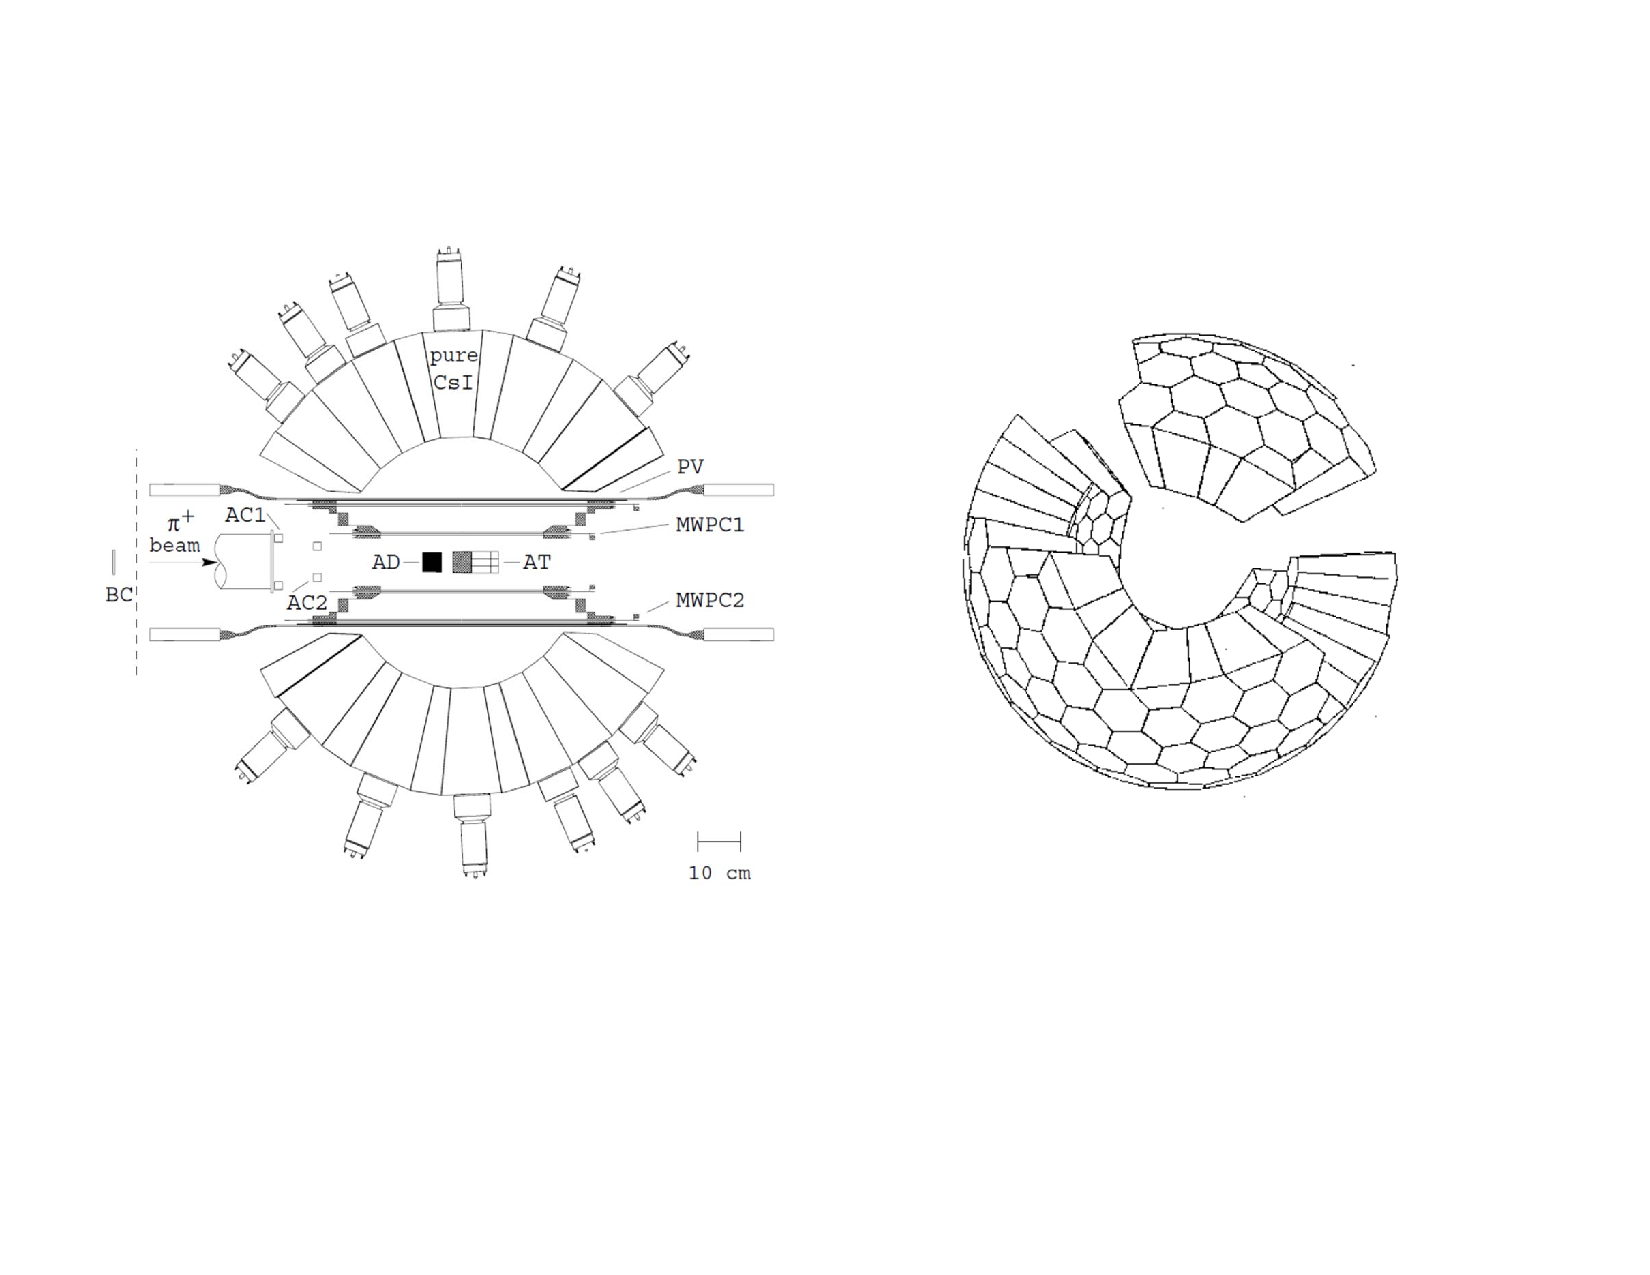
\includegraphics[scale=0.6]{sections/figures/PEN figure.pdf}
\vspace{-40mm}
\caption{Left: PEN detector. Right: Cutaway view of the PEN CsI crystal spectrometer\cite{Pocanic1,Pocanic2,Pocanic6}.}
\label{fig:PEN}
\end{figure}
